% Created 2021-09-08 Wed 15:31
% Intended LaTeX compiler: pdflatex
\documentclass[11pt]{article}
\usepackage[utf8]{inputenc}
\usepackage[T1]{fontenc}
\usepackage{graphicx}
\usepackage{grffile}
\usepackage{longtable}
\usepackage{wrapfig}
\usepackage{rotating}
\usepackage[normalem]{ulem}
\usepackage{amsmath}
\usepackage{textcomp}
\usepackage{amssymb}
\usepackage{capt-of}
\usepackage{hyperref}
\author{Jonatan Ahumada \& Jorge Garzón}
\date{\today}
\title{Becos}
\hypersetup{
 pdfauthor={Jonatan Ahumada \& Jorge Garzón},
 pdftitle={Becos},
 pdfkeywords={},
 pdfsubject={},
 pdfcreator={Emacs 27.2 (Org mode 9.4.6)}, 
 pdflang={Spanish}}
\begin{document}

\maketitle
\tableofcontents



\section{Análisis del entorno}
\label{sec:org0a2d41b}
\subsection{PESTEL}
\label{sec:org03a0191}
\subsubsection{Político}
\label{sec:org29b85a6}
\begin{enumerate}
\item Amenaza de variante delta y mu
\label{sec:orga13095c}

Con la aparición de nuevas variantes, la comunidad internacional está
considerando volver a implementar medidas de aislamiento.

Esto es una \textbf{amenaza} porque la infraestructura física requiere un
plantel de trabajadores para sus procesos de confección, que está
ligado a la mano de obra de las trabajadoras. Habra más costos para
garantizar la salubridad y hay límites de espacio que se deben
respetar, lo que disminuye capacidad de producción

\item Cese de presencialidad en los colegios
\label{sec:org5978d9b}

Si se prolonga el aislamiento social, por un posible cuarto pico, la
proyección de ventas se desploma, puesto que prinipalmente recae en
escuelas de futbol y colegios de Bogotá, que participan en torneos
locales.

Esto es una \textbf{amenaza} porque no habrá demanda de uniformes por
parte de ese segmento.


\item Déficit fiscal y tributación de la reforma 2.0:
\label{sec:orgde015ff}

En la nueva reforma fiscal la tarifa de renta subirá del 30 al 35\%
para hacerle frente al déficit fiscal que enfrenta el país.

Esto es una \textbf{amenaza} porque los márgenes de rentabilidad será más
estrecho.  Más aun, teniendo en cuenta el costo competitivo que el
plan de negocios plantea para sus productos.
\end{enumerate}

\subsubsection{Económico}
\label{sec:org500d3b4}
\begin{enumerate}
\item Alsa del dólar
\label{sec:orga063f33}
La amenaza de la variante delta hace que la Fed aumente las tasas de
interés del dolar, lo que desvaloriza el peso colombiano frente a la
divisa.

Esto es una \textbf{amenaza} porque puede disuadir la inversión extranjera
en el sector textil. Esto puede reducir los márgenes de
rentabilidad de la confección, manufactura y distribución
de producto textil.

\item Proceso de reactivación económica
\label{sec:org28a33b2}
\end{enumerate}
\subsubsection{Social}
\label{sec:orgd702a4a}
\begin{enumerate}
\item Protagonismo del sector textil colombiano a nivel internacional
\label{sec:org67929b6}

El sector textil y la moda registra el 37\% de las empresas registrados en CCB.
Según Colombia Productiva, el sector textil y de confección es el primer
generador de mano de obra en la industria nacional. Además, Colombia es el
primer exportador de tejido plano en Suramérica.

Esto es una \textbf{oportunidad} porque el reconocimiento externo de la moda colombiana
podría formar sinergía con una de las propuestas diferenciadoras de Becos:
ayudar a madres cabezas de hogar de sectores vulnerables a la vez que se
contribuye al medio ambiente, dado que estos son temas coyunturales.

\item Necesidad de impulsar la reactivación económica
\label{sec:orgac7ebb8}

El Gobierno Duque enfatiza que el pais muestra ritmo de crecimiento
elevado (1,1\%) el primer trimestre del año, en comparación con paises
como Chile o México. El gobierno pronostica un desarrollo favorable
durante el resto del año.

Esto es una \textbf{oportunidad} porque parece improbable que el gobierno
actual paralice la reactivación ecónomica, más aún si se se han hecho
esfuerzos presupuestales para iniciar le proceso de vacunación.
\end{enumerate}

\subsubsection{Tecnológico}
\label{sec:org20fde08}
\begin{enumerate}
\item Costos en servicios web
\label{sec:org049bc4a}
Los servicios de Cloud Computing de Amazon se cotizan en dólares.
Este servicio es parte crucial de la infraestructura tecnolgócia

Esto es una \textbf{amenaza} porque aumenta los costos en infraestructua
\item Escasez de profesionales TI
\label{sec:org0ee58e0}

Esto es una \textbf{amenaza} heredada del mercado de talento humano
colombiano, ya que a día de hoy existe una demanda superior a la
oferta en cuanto a profesionales TI.
\end{enumerate}

\subsubsection{Ambiental}
\label{sec:orge550e3f}
\begin{enumerate}
\item Aceptación cultural del reciclaje
\label{sec:org3ae5347}
El mundo está entrando en periodo de conciencia ambiental. En
Colombia, sectores como el de los hidrocarburos están iniciado una
transformación hacia energías más limpias.

Esto es una \textbf{oportunidad}, puesto que hay una tendencia cultural
por participar en la genereción de un mundo ecosostenible, lo
que hace que la propuesta de Becos altamente atractiva en el pais
y el mundo por igual.
\end{enumerate}
\subsubsection{Legal}
\label{sec:orgb9b1272}
\begin{enumerate}
\item Beneficios de una Sociedad por acciones simplificada
\label{sec:org1303f7f}

En Colombia, estar constituido de esta manera representa una
\textbf{oportunidad}, dadas las exenciones tributarias que conlleva.

\item Beneficios ambientales
\label{sec:org39768c3}

Se considera una \textbf{oportunidad} ya que la propuesta de Becos también
pretende ser referente a nivel de leyes.
\end{enumerate}
\subsection{5 Fuerzas}
\label{sec:orgb678fca}
\begin{figure}[htbp]
\centering
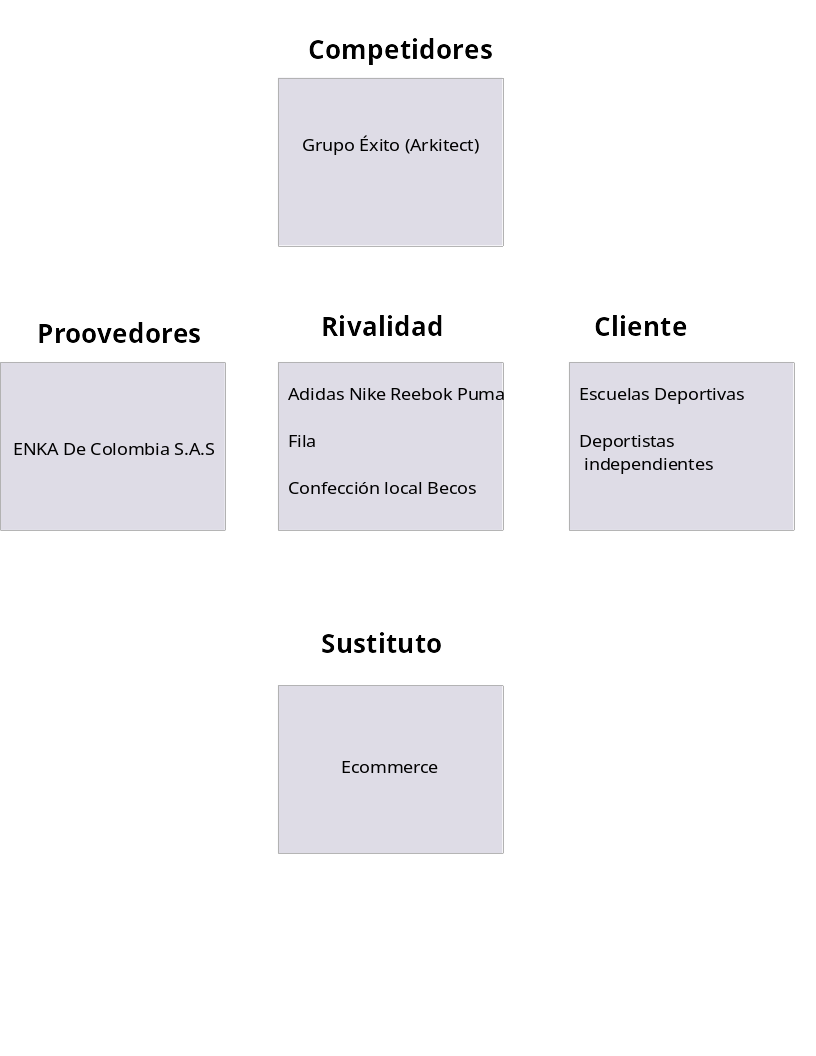
\includegraphics[width=.9\linewidth]{./assets/build/5_fuerzas.png}
\caption{\label{fig:org7c89b21}5 fuerzas de Porter}
\end{figure}

\section{BMM}
\label{sec:org090a46c}
\subsection{Misión y vision}
\label{sec:org7d9b109}
\subsubsection{Misión}
\label{sec:orgd83d000}
Ser referente nacional e internacional con respecto
a procesos ecologicamente sostenibles en el sector
textil. Unir el diseño de la moda colombiana
con la sostenibilidad y la conciencia social.

\subsubsection{Visión}
\label{sec:org5347890}

Para el año 2025, BECOS tendrá toda todo un catálogo de ropa deportiva
fabricada con elementos 85\% reciclados. Tendrá lineas de ropa deportiva para
todos los deportes que demanden indumentaria deportiva, desde los más
practicados por los colombianos: fútbol, basquetból, ciclismo, tenis, entre
otros, hasta los de díficil adquisición: danza, ballet, patinaje,
deportes urbanos etc.

\subsection{Assesment}
\label{sec:org02d7518}
\begin{enumerate}
\item Influencias
\label{sec:orgc53e3eb}

\begin{enumerate}
\item Externas

\begin{itemize}
\item Gobierno Colombiano
\item Mercado Internacional
\item Confeccionistas de Bogotá
\end{itemize}
\end{enumerate}


\begin{enumerate}
\item Internas

\begin{itemize}
\item Adecuación a protocolos de Bioseguridad
\item Implementación de hardware y software
\end{itemize}
\end{enumerate}

\item DOFA
\label{sec:orgb240747}
\begin{figure}[htbp]
\centering
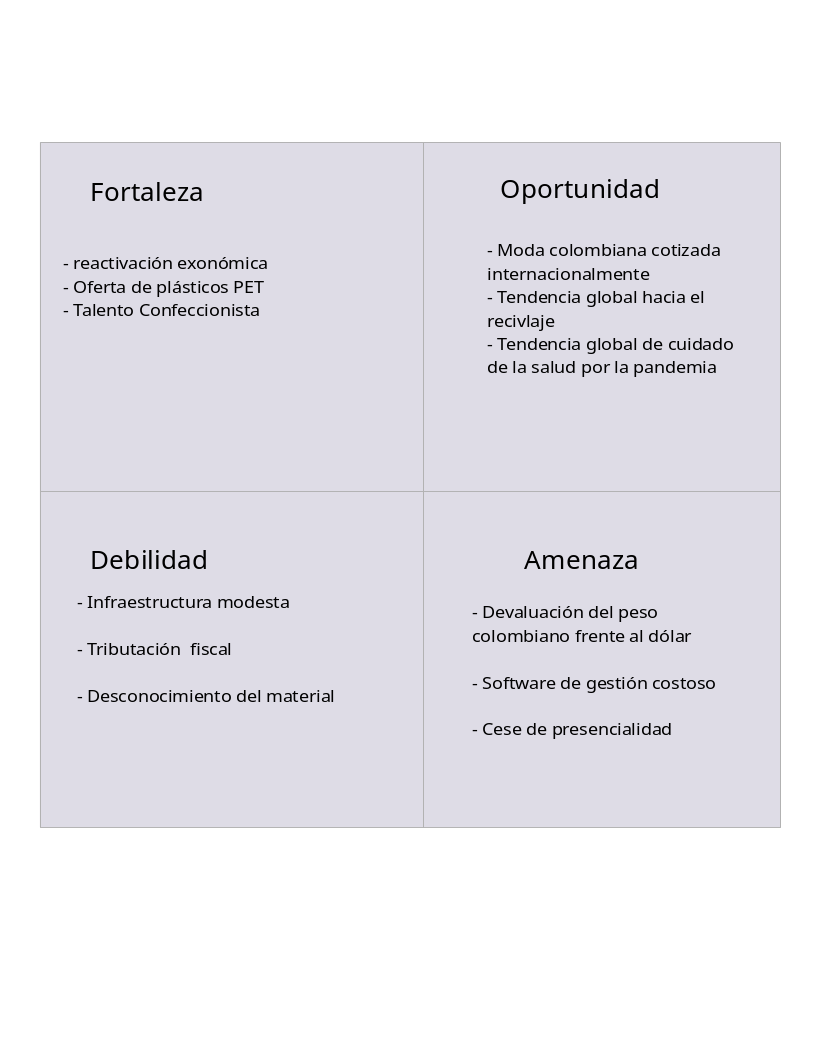
\includegraphics[width=.9\linewidth]{./assets/build/dofa.png}
\caption{\label{fig:org2cd12fa}DOFA para Assesment de Influencias}
\end{figure}
\end{enumerate}


\subsubsection{Medios}
\label{sec:org776dd74}

\begin{figure}[htbp]
\centering
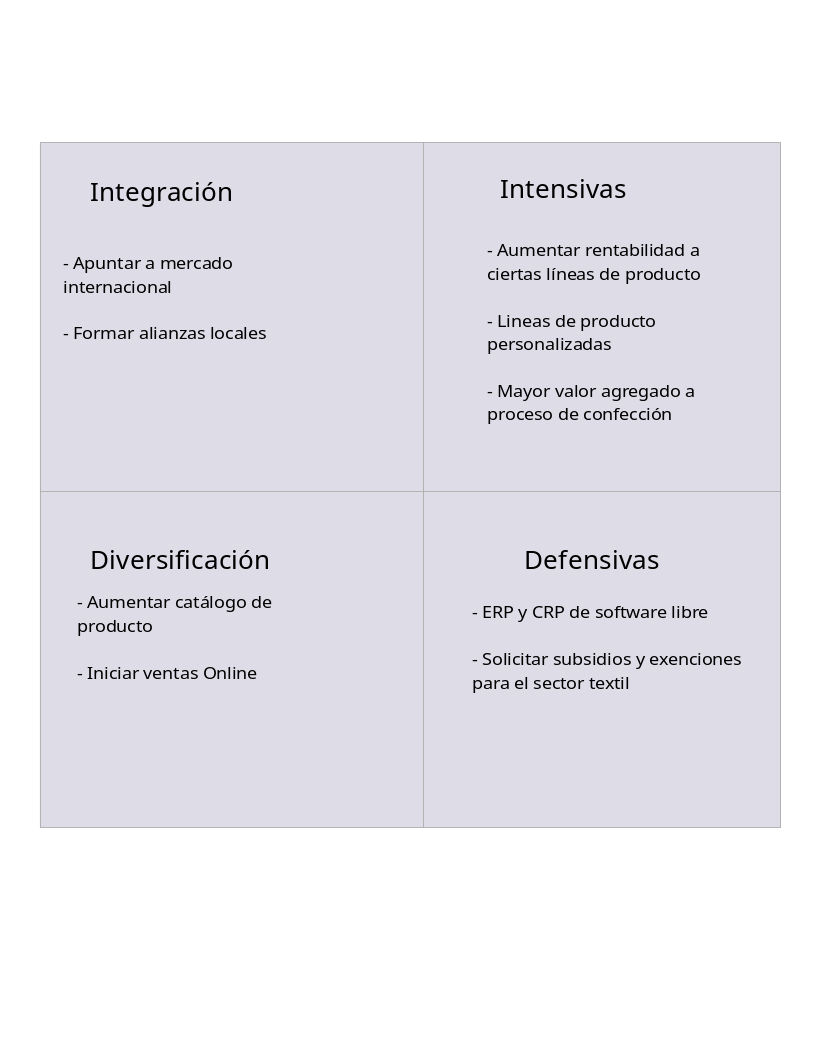
\includegraphics[width=.9\linewidth]{./assets/build/means.png}
\caption{\label{fig:org029773d}Estrategia}
\end{figure}

\subsubsection{Externas}
\label{sec:org020969c}

\subsection{Blue Ocean Strategy Canvas \& ERRC GRID}
\label{sec:orgeb48be3}
\begin{figure}[htbp]
\centering
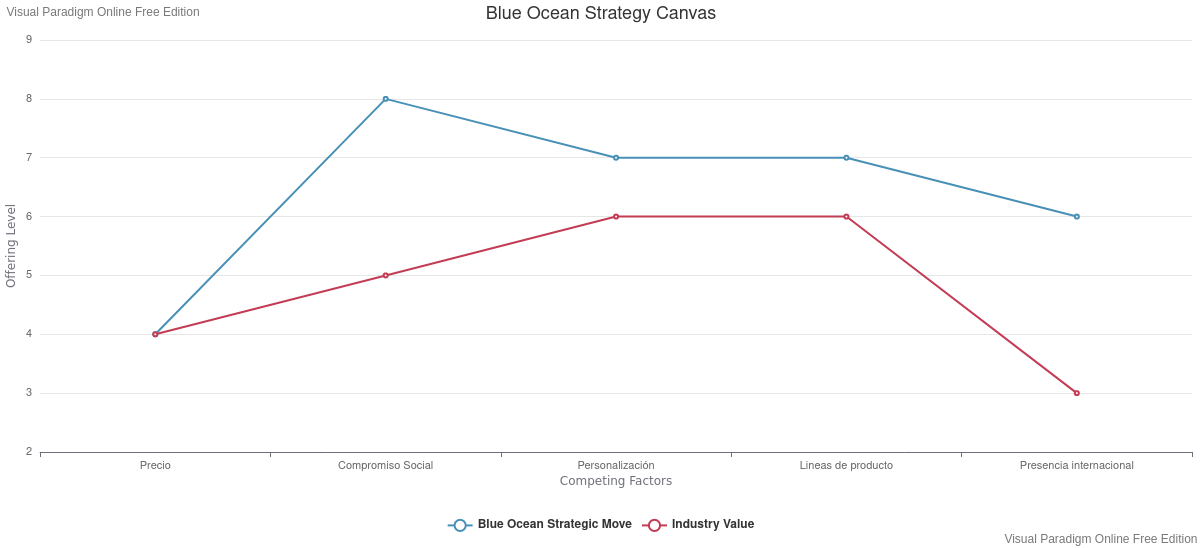
\includegraphics[width=.9\linewidth]{./assets/build/blue_ocean_canvas.png}
\caption{\label{fig:org95657a5}Blue Ocean Strategy Canvas}
\end{figure}
\begin{figure}[htbp]
\centering
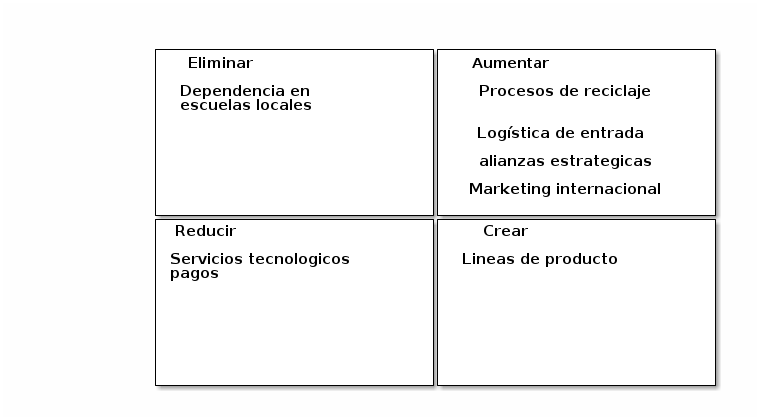
\includegraphics[width=.9\linewidth]{./assets/build/ercc.png}
\caption{\label{fig:orga751ab0}ERRC}
\end{figure}
\subsection{Mapa de procesos, diccionario de procesos y organigrama}
\label{sec:orgcf047ed}
\begin{figure}[htbp]
\centering
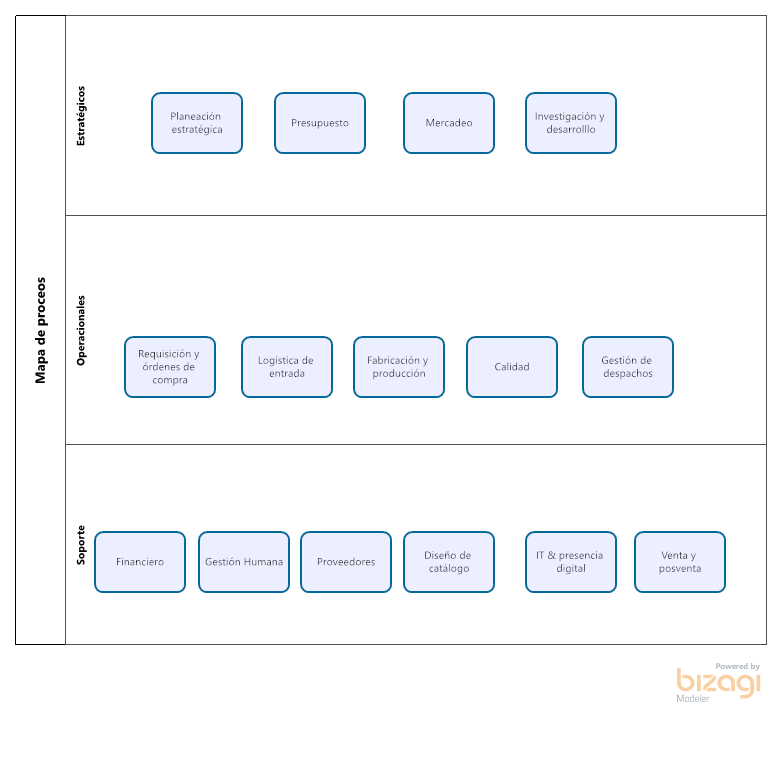
\includegraphics[width=.9\linewidth]{./assets/build/mapa_procesos.png}
\caption{\label{fig:org85bcfbc}Mapa de procesos}
\end{figure}

\begin{figure}[htbp]
\centering
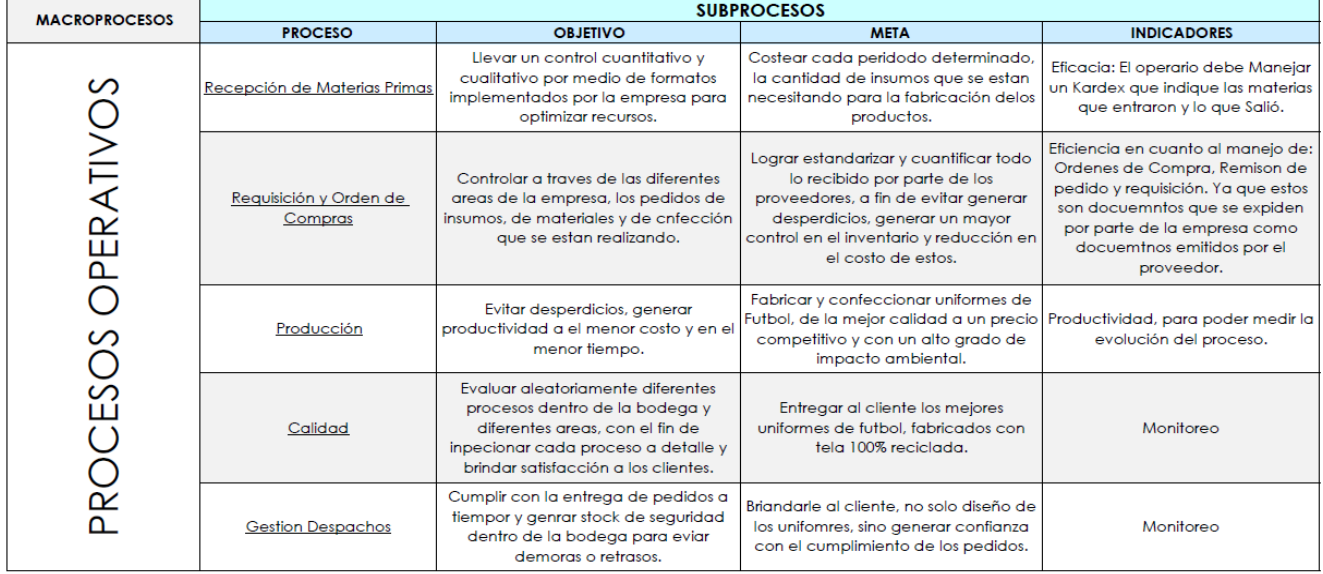
\includegraphics[width=.9\linewidth]{./assets/build/diccionario_procesos.png}
\caption{\label{fig:org2565212}Diccionario de Procesos}
\end{figure}

\begin{figure}[htbp]
\centering
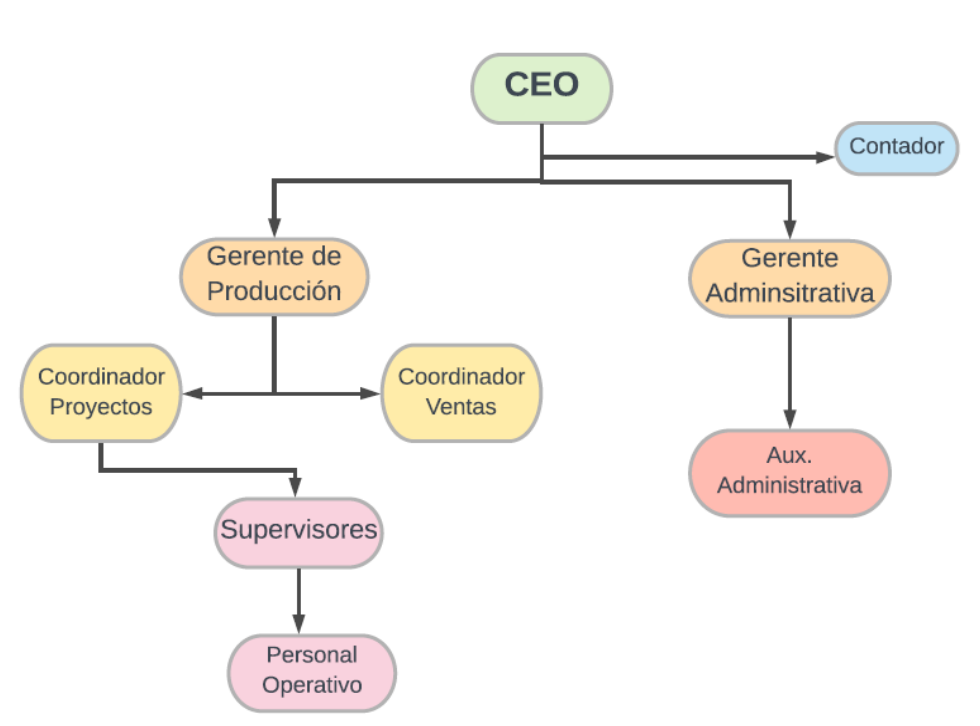
\includegraphics[width=.9\linewidth]{./assets/build/organigrama.png}
\caption{\label{fig:orgbe62c93}Organigrama}
\end{figure}

\section{Buyer Persona}
\label{sec:org12fddb8}
\subsubsection{Definición del segmento de clientes}
\label{sec:orga9b4ae6}
Los clientes potenciales de BECOS son principalmente
dos segmentos.

\begin{enumerate}
\item Padres de niños en escuelas de fútbol

El segmento principal de BECOS son
las escuelas de fútbol, puesto
que presentan la necesidad
de adqirir un uniforme.
Sin embargo, en este momento
este segmento está en amenaza,
por las restricciones en la
presencialidad de los colegios
y la prohibición de aglomeraciones.
Aunque el usuario final es un niño
o joven menor de 18, los clientes
son padres de un rango variable de
edad.
\end{enumerate}


\begin{enumerate}
\item Deportistas de equipos independientes 

En Bogotá se observa que las
canchas de los parques públicos se utilizan
para jugar extra-oficialmente. Es decir,
sin necesidad de estar inscritos en una
escuela. Por lo general, los usuarios
forman equipos regulares de amigos, o
conocidos del área que podrían estar
interesados en adquirir un uniforme,
para añadir un 'plus' a sus partidos
recreaionales.

\begin{enumerate}
\item Deportistas individuales

Junto a los deportistas que juegan en grupos
de amigos, se observa que hay también un
segmento considerable de personas que
realizan actividades deportivas de manera
individual y que pueden tener necesidad
de un producto confeccionado a la medida.
Por ejemplo, personas que trotan, que
entrenan con entrenador personal, que
realizan ejercicios de calistenia, etc.
\end{enumerate}
\end{enumerate}



\subsubsection{Entrevistas}
\label{sec:orga1d90d9}
En este momento, solo contamos con una entrevista:

\begin{verbatim}
Jorge Garzón: Cuando jugaba futbol, ¿Lo hacía de manera aficionada o por algún torneo?

Entrevistado: Ambas.

JG: ¿Con uniforme?

E: Sí, claro.

JG: ¿Cuánto fue lo máximo que pagó por un uniforme?

E: En ese tiempo, aproximadamente $50.000 o un poco más.

JG: ¿Se ponían de acuerdo?

E: La mayoría lo hacía.

JG: ¿Siempre estuvo satisfecho con esas decisiones?

E: La mayoría de las veces, y uno accedía con tal de estrenar uniforme.

JG: ¿Le quedaba bien el uniforme?

E: Sí

JG: ¿Y al momento del partido?

E: Sí

JG: ¿Le parecía justo el precio?

E: Mire que sí. Lo mandábamos a hacer en Saeta y Speed.

JG: En su momento, ¿Hubiera pagado más por tener más opciones de personalización en su uniforme?

E: Sí, claro.

JG: ¿Le prestaba atención al material de su uniforme?

E: Sí, claro.

JG: ¿Y si su uniforme fuera hecho con plástico PET?

E: No sé, se suda más uno y se acalora más, ¿no? Por eso uno los manda a hacer en tela, ya que siente más brisa.

En este punto, se le explicaron los beneficios de hacer un uniforme mediante plásticos PET.

E: Igual sería bacano, ya que se utiliza mayor material reciclado

JG: ¿Algún confeccionista le presentó opciones de personalización?

E: No

JG: ¿Le parece interesante cotizar uniformes por internet y luego ir a la fábrica?

E: Sí, claro.
\end{verbatim}
\subsubsection{Encuesta}
\label{sec:org1cb14e1}

\begin{verbatim}
Aspectos del producto    
- ¿juegas en algún equipo de fútbol, tienen uniformes?
- ¿Tuviste alguna capacidad de decisión en cuanto al uniforme de tu equipo?
- ¿Quien te pareció que tuvo el factor decisivo en la decisión?
- ¿Estuviste de acuerdo con la decisición del uniforme?
- ¿Estás satisfecho con la calidad de tu uniforme?
- ¿Te orma bien tu uniforme?
- Si no, ¿qué le mejorarías?
- ¿Te gusta estéticamente tu uniforme?
- Si no, ¿qué le mejorarías?
- ¿Te parece justo el precio que pagaste por los uniformes que has comprado?
- ¿Te parece que un precio entre  45,000 y 48,000  es competitivo para un uniforme (camisa y pantaloneta) en Bogotá?
- ¿Pagarías más para tener más opciones de personalización en tu uniforme?
- ¿Pagarías más para tener un tejido más resistente en tu uniforme?

factor diferenciador 
- ¿Le prestas atención al material del uniforme, sabes de qué estan hechos los uniformes que has comprado anteriormente?
- ¿Conoces los beneficios del PET como tejido textil?
- Ahora que los conoces (se los dices):
- ¿Te importaría positivamente si los uniformes están hechos con un alto grado de plastico PET desechable para contruibir al planeta?
- ¿Te importaría negativamente si los uniformes están hechos con un alto grado de plástico PET desechable para contribuir al planeta?
- ¿Conoces cómo confeccionaron los uniformes que has comprado anteriormente?
- ¿Te importaría positivamente si los uniformes están confeccionados por madres cabeza de hogar?
- ¿Te importaría negativamente si los uniformes están confeccionado por madres cabeza de hogar?
- ¿Te interesaría tener uniformes para jugar con tus amigos (torneos no oficiales, fines de semana, etc?
- ¿Te interesaría poder diseñar uniformes?
- ¿Te interesarí ir a premisas (a la fabrica), para comprobar tonalidades de color y medidas de la prenda antes de producir el producto?
- ¿Has comprado algun uniforme que te ofrezca personalización anteriormente?
- ¿Has comprado a algún confeccionista en Bogotá que te ofrezca validación de colores y medidas antes de comprar el uniforme?

diversificacion
- ¿Te interesaria cotizar uniformes por internet y luego validarlos en premisa?
- ¿Te interesaria participar en eventos deportivos auspiciados por BECOS y otros sponsors?
- ¿Te interesaria tener otros productos de un material similiar y estética al de tu uniforme?
- ¿Puedes nombrar alguno que te interese (buzos, gorras, bolsos, etc, ropa casual)?


\end{verbatim}


NOTA: hay más encuestas realizadas (7), pero
la transcripción aún no se ha realizado
\subsubsection{Cliente incognito}
\label{sec:org3d2d919}

Pendiente.

\subsubsection{Observación}
\label{sec:org409d903}

Alrededor de las escuelas de fútbol se forma una microcomunidad en la que un
grupo significativo de padres participa. Esta comunidad se identificó como
un segmento y posteriormente se hizo un \emph{buyer persona}. Es un blanco
potencial a explotar, aunque es difícil encaminar los esfuerzos porque
sencillamente no reportan tener una injerencia en la decición de compra en
los uniformes.

Los entrenadores, por su parte, que serían siendo un cliente más directo de
Becos. Sin embargo, están constantemente apurados con el tiempo o atendiendo
a los padres. La entrevista es difícil y apurada. El uniforme tiende a
representar los valores de la escuela y muestran una actitud cerrada a la
idea de personalización y mayor participación de padres o confecionistas.


Sin embargo, las entrevistas revelan que hay aspectos de la indumentaria
deportiva con los que hay insatisfacción y que los entrenadores simplemente
desconocen y no tendrían tiempo de abordar.

Principalmente, las madres reportan que la amplitud de los uniformes no es
favorable para sus hijas, que ls gustaria que se secaran más rapido y
exiguieran menos cuidado, que fueran más resistentes y tuvieron una
respuesta muy positiva al precio.

Un grupo considerable siente insatisfacción con la estética del uniforme,
aunque manifiestan que no hay nada que se pueda hacer, porque es
prerrogativa del colegio o institución.




\subsubsection{Identificacion y definición de los clientes}
\label{sec:org1d5c8de}

Hasta ahora se han distinguido tipos de clientes,
que corresponserán a 3 segmentos:

\begin{enumerate}
\item Madres y padres de familia (cliente)

\item Menor de edad deportista (consumidor final)

\item Entrenadores y directivos de escuelas de futbos (cliente)

\item Jugadores/Deportistas de equipos independientes (clientes)

\item Jugadores/Deportistas individuales (cliente)
\end{enumerate}



\section{Buyer Personas}
\label{sec:org3895450}

Los Buyer personas se hicieron a partir de la identificción de los
clientes y las entrevistas. 

\subsection{Adri}
\label{sec:orgacbdbe4}

\begin{verbatim}
'Adri' 

Segmento

Padres de familia

Puesto 

Representante de venta 

Edad 

Entre 35 y 44 años 

Nivel de educación más alto 

Título profesional 

Redes sociales 


Industria 

Publicidad 

Tamaño de la organización 

Entre 1 y 10 empleados 

Canal favorito de comunicación 


Teléfono 
Correo electrónico 
Herramientas que necesita para trabajar 


Sistemas de gestión de contenido 
Gestión de proyectos 
Responsabilidades laborales 

Dirigir grupos pequeños de personas 

Su trabajo se mide en función de 

productividad 

Su superior es 

Director 

Metas u objetivos 

Sacar más tiempo para su familia y mantener un empleo satisfactorio 

Obtiene información a través de 

De su formación profesional y red de contactos 

Dificultades principales 


Gestión de proyectos y falta de organización 
Colaboración y creatividad 
Frustraciones 

No siente que su labor como madre es reconocida, a pesar de que es muy dedicada. 
Semanalmente acompaña a su hijo la escuela de fútbol y participa mucho en las actividades de la 
escuela. Sin embargo, esto la obliga a manejar muy buen su tiempo porqe tiene un ritmo de 
trabajo considerable. 

¿Qué escucha? 

Escucha que hay muchos problemas en el mundo y siente que debe colaborar con el cuidado 
medioambiental y sectores menos privilegiados. Sus amigas tienen u estilo de vida diferente al 
de ella (algunas no están casadas), pero ella prefiere priorizar su hogar y luego, desempeñarse 
bien en el mundo laboral. Entiende que su hijas están expuestas a retos insospechados y por eso 
les brinda el mejor acompañamiento posible, sin ser sobreprotectora. 
\end{verbatim}

\subsection{Entrenador Richard}
\label{sec:org039bf84}




\begin{verbatim}

Entrenador Richard 

Segmento

Entrenadores

Puesto 


Entrenador Líder 

Edad 

Entre 35 y 44 años 

Nivel de educación más alto 

Licenciatura 

Redes sociales 


Industria 

Cuidado de la salud 

Tamaño de la organización 

Entre 11 y 50 empleados 

Canal favorito de comunicación 


Teléfono 
Correo electrónico 
Herramientas que necesita para trabajar 


Correo electrónico 
Responsabilidades laborales 

Escribe aquí 

Su trabajo se mide en función de 

Supervisión de los horarios de entrenamiento, interacción con padres y alumnos, mide el 
resultado de entrenadores a su cargo, consigue eventos deportivos para que los alumnos 
puedan participar 

Su superior es 

Dueños de la escuela privada de fútbol 

Metas u objetivos 

Richard ha sido entrenador durante mucho tiempo en la escuela, y esta ha adquirido gran 
prestigio, por lo que siente gran orgullo. Cree en los valores de la disciplina y el trabajo y 
procura comunicarselos a sus alumnos. 

Obtiene información a través de 

En su formación profesional 

Dificultades principales 


Moral del empleado a cargo y de los muchachos

Gestión del cambio

Frustraciones 

Richard maneja varios grupos de entrenamiento (de 3 a 5) todos los días , incuidos los sábados. 
Debe mantener una actitud positiva todo el tiempo, pero en ocasiones es difícil lidiar con los 
padres. El entiende que están preocupados por sus hijos, pero a la vez se da cuenta de que 
muchos los sobreprotejen. Debe balancear la complacencia hacia padres y alumnos con la 
excelencia deportiva. 
\end{verbatim}


\subsection{Jason Rappiazone}
\label{sec:org992ae0e}

\begin{verbatim}
Jason Rappiazone 

Segmento

 Jugadares regulares independientes

Puesto 

Mensajero en diferentes empresas 

Edad 

Entre 18 y 24 años 

Nivel de educación más alto 

Secundario o equivalente 

Redes sociales 


Industria 

Alimentos y bebidas 

Tamaño de la organización 

Trabajador independiente 

Canal favorito de comunicación 


Mensajes de texto 
Teléfono 
En persona 
Redes sociales 
Herramientas que necesita para trabajar 

Smartphone, bicicleta eléctrica 

Su trabajo se mide en función de 

Por envíos 

Responsabilidades laborales 

Hacer envíos a tiempo. 

Metas u objetivos 

Jason aspira un mejor nivel salarial, que le permita dedicarse a algo que le apasione, aunque aún 
no ha hallado qué es. Hay situaciones socioeconocimas que se han interpuesto en su camino, por 
lo que lleva algunos años trabajando como mensajero para varias empuestas. 

Su superior es 

Director 

Obtiene información a través de 

Del contancto con otros jóvenes como el.

Dificultades principales 


Desarrollo profesional 
Recursos 

Frustaciones 

Siente que la vida a sido injusta con el y que a otras personas les ha tocado mucho más fácil. Por 
eso siente un vínculo bastante fuerte con otros jóvenes que laboran en los mismos trabajos que 
el. Anda mucho en la calle y las interacciones sociales son importantes durante el dia. 
El fútbol luego del trabajo es pan de cada día. 


¿Qué escucha? 

Ve muchas redes sociales porque trabaja con su smartphone. Ve muchos contenidos de 
recreación, como con 'Con Ánimo de Ofender', pero tambien se siente muy atraido por las 
protestas sociales, que abundan en el país, y en países aledaños. 
\end{verbatim}
\end{document}
